\documentclass[10pt, a4paper,english,spanish]{article}
%\documentclass[10pt,a4paper]{article}
\usepackage[utf8]{inputenc} % para poder usar tildes en archivos UTF-8
\usepackage[spanish]{babel} % para que comandos como \today den el resultado en castellano
\usepackage[conEntregas]{caratula}
\usepackage{fullpage} %small margins
\usepackage[parfill]{parskip} %genera saltos entre parrafos
\usepackage{color}
\definecolor{gray}{gray}{0.35}
\usepackage{listings}
\usepackage{enumitem}
\usepackage{soul}
\usepackage{amsmath} %big brackets
\usepackage[pdftex]{graphicx}
\lstset{
    numbers=left,
    breaklines=true,
    tabsize=2,
    basicstyle=\ttfamily\color{gray},
}
\setlength{\parindent}{8pt}
\usepackage{mathtools}
\usepackage[margin=50pt]{geometry}
\usepackage{amsfonts}
\usepackage{flafter}
\usepackage{multicol}
\usepackage{caption}
\usepackage{subcaption}
\usepackage{graphicx}
\setlength{\parindent}{0pt} %remueve indent

%paquete para setear colores a las tablas para graficar registros
\usepackage{xcolor,colortbl}
%define de colores
\definecolor{Orange}{rgb}{1, 0.64, 0}
\definecolor{Green}{rgb}{0.32,1,0.62}
%\definecolor{Purple}{rgb}{0.44,0.20,0.81}
%define de columnas
\newcolumntype{o}{>{\columncolor{Orange}}c}
\newcolumntype{g}{>{\columncolor{Green}}c}
%\newcolumntype{p}{>{\columncolor{Purple}}c}
%holi
\begin{document}

\materia{Organización del Computador II}
\submateria{Trabajo Práctico Nro. 3}
\titulo{Informe - Grupo: SnakeII/Nokia1100}
\fecha{\today}
\integrante{Pablo Gomez}{156/13}{mago-1986@hotmail.com}
\integrante{Lucía Parral}{162/13}{luciaparral@gmail.com}
\integrante{Petr Romachov}{412/13}{promachov@gmail.com}
\maketitle
\newpage

\tableofcontents

\newpage
% Comienzo Introducción
\section{Introducción}
En este trabajo práctico se busca experimentar con el procesamiento con instrucciones SIMD que operan con múltiples datos simultáneamente.\\ 
Con este fin, desarrollamos distintas implementaciones de los filtros Blur, Merge y HSL sobre imágenes y evaluamos su rendimiento.\\
\subsection{Sobre la experimentación}
Realizamos las experimentaciones para los tres filtros con sus respectivas implementaciones de la manera detallada a continuación.\\
Para realizar casos de tests exhaustivos, utilizamos imágenes de distintos tamaños y tipos.
Tomamos imágenes de colores constantes (es decir, imágenes totalmente blancas, azules, verdes, rojas y negras), imágenes que tienden a estos colores e imágenes mixtas.
Cada una de estas imágenes las procesamos en los tamaños 40x40 (1600 píxeles), 300x300 (90000 píxeles) y 600x600 (360000 píxeles), ya que nos pareció una variación razonable para mostrar la performance de las distintas implementaciones de los filtros.\\
Para cada filtro y cada implementación, calculamos la cantidad de ciclos de clock que transcurren en las instrucciones que procesan la imagen (obviando la carga de la misma y el guardado de datos). Para medir los ciclos de clock usamos las funciones provistas por la cátedra en el archivo rdtsc.h. 
Teniendo en cuenta que existen problemáticas al momento de conocer el tiempo de ejecución real de los programas, ya que la ejecución puede ser interrumpida por el scheduler para realizar un cambio de contexto o bien que los procesadores varían la frecuencia de reloj, ideamos la siguiente metodología para medir la cantidad de ciclos de clock de nuestras implementaciones: para cada test entonces, realizamos 100 repeticiones, tomando el promedio de los resultados obtenidos.\\ Luego, descartamos el 10\% de los peores casos. Una vez hecho esto, calculamos el desvío estándar del 90\% de los casos restantes. De esta forma, obtuvimos un resultado promedio, y sumando y restando a este valor el desvío estándar, el resultado esperado en mejor y peor caso. Así mismo, el desvío estándar también nos sirve como indicador de qué tan precisas fueron las mediciones.\\
Además, compilamos las implementaciones de C provistas por la cátedra con el parámetro de compilación -O3, que aseguraba la versión más optimizada del código, para poder acercarnos a la mejor ejecución posible de dichas implementaciones.\\

%TODO: Calcular o chamuyar el desvío estándar en las mediciones y hablar un poco de eso luego.

Cabe destacar que la computadora en la que realizamos las experimentaciones cuenta con las siguientes especificaciones técnicas:\\
%TODO: Agregar características técnicas de la computadora del Mago

Para experimentar acerca de si variaba el rendimiento de una implementación en función del tipo de imagen testeado elaboramos la siguiente estrategia. Agrupamos los distintos tipos de imágenes con los que contábamos como casos de prueba, descritos en la introducción del apartado de experimentación, y tomamos el promedio de tiempos de ejecución (tomando el 10\% peor como outliers) para cada subgrupo. Luego, tomando los promedios de cada tipo de imagen como el representante de dicho tipo, calculamos el desvío estándar entre todos los representantes. Una vez calculado el desvío estándar, lo dividimos por el promedio y multiplicamos por 100 para tener un “porcentaje de desviación”. De esta forma, un porcentaje elevado significa que los representantes de cada tipo de imagen difieren significativamente, mientras que un porcentaje pequeño, que todos los representantes estan cercanos al promedio y por lo tanto, las mediciones dentro de todos los tipos se mantiene estable.\\

Por último, tomamos como decisión para una mayor claridad en los gráficos, el utilizar escala logarítmica para representar los ciclos de clock, ya que de no hacerlo, se perdía claridad y representatividad en los mismos. De cualquier manera, en cada gráfico figurará qué tipo de escala está utilizando, y cualquier otra información relevante.
A continuación, describiremos para cada filtro su desarrolo, los resultados obtenidos y el análisis comparativo en relación con las implementaciones que realizamos y otras posibles.\\\\\\\\\\\\\\\\\\

% \begin{figure}[ht]
% \centering
% 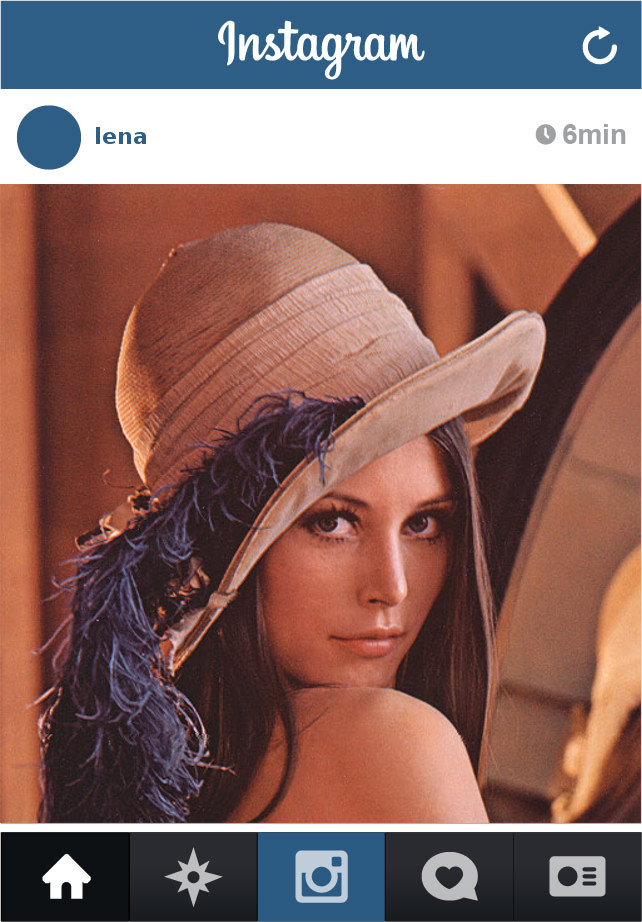
\includegraphics[width=90mm]{introduccion/lena_instagram.jpg}
% %\caption{A simple caption \label{overflow}}
% \end{figure}

% Fin Introducción

\newpage
% Comienzo Ejercicio 1
\section{Ejericio 1}

\subsection{Completar la tabla de descriptores globales}
Para esto completamos el indice 0 de la GDT con el descriptor nulo. Las siguientes 7 entradas por requerimientos de este trabajo debian ser nulas.
A continuación, completamos con entradas para código y datos para sistema operativo (nivel 0) y para usuario (nivel 3). Los segmentos de código y datos del sistema operativo están descritos en las entradas 8 y 9 respectivamente, mientras que los de usuario en las entradas 10 y 11. 
El campo límite para estas entradas es 0xF3FF y la base 0x0000, con granularidad 1, ya que direccionan  500MB de memoria. El tipo para los los descriptores de código es 0x8, correspondiente a código de sólo-ejecución, mientras que para los de datos es de 0x2, para segmentos de datos de lectura/escritura. También es relevante indicar que para todas estas entradas, el campo p es 1, ya que los segmentos se encuentran presentes.
También tenemos una entrada de datos para el segmento de video, con base 0xB800 y límite 0xC0000, con dpl 0, pues es para ser utilizado sólo por el kernel, presente y permisos de lectura/escritura. Este descriptor tendrá índice 12. 

\subsection{Pasaje a modo protegido}
En primer lugar, cambiamos el modo de video a 80x50.
Habilitamos a20 llamando a \texttt{habilitar\_A20}.
Cargamos la GDT  con la instrucción \texttt{lgdt}.

Para pasar a modo protegido, seteamos en 1 el bit PE del registro CR0 y hacemos jump far con un selector de segmento de código de nivel 0 y offset \texttt{modo\_protegido} (etiqueta que declaramos a continuación)

Una vez en modo protegido, asignamos los selectores de segmentos. Como ds, ss elegimos segmento de datos de nivel 0, y para fs el segmento de video.

Seteamos la pila del kernel en la direccion 0x27000.

\subsection{Inicialización de la pantalla}

Para esto tenemos la función \texttt{screen\_inicializar}, que pinta el fondo de gris, y el recuadro para cada jugador en azul y rojo.

% Fin Ejercicio 1

\newpage
% Comienzo Ejercicio 2
\section{Ejericio 2}

\subsection{Creación de las estructuras de la IDT} 

En la función \texttt{idt\_inicializar} inicializamos las entradas iniciales de la IDT (de la 20 a la 31 estan reservadas para Intel).\\\\
Ademas inicializamos las entradas 32 para reloj, 33 para teclado y 70 para las syscalls a ser utilizadas por las tareas.\\\\
Las entradas de la IDT estan definidas por una macro en la que elegimos el número que representa su índice.\\ 
A la entrada para la syscall le damos los siguientes atributos: 0xEE00.\\
A todas las demás: 0x8E00.\\


Estas difieren ya que la syscall al ser llamada por la tarea, necesita tener dpl = 3 para que esta pueda accederla, mientras que las otras interrupciones no.\\

Luego para que el procesador utilice la IDT utilizamos la interrupción lidt y configuramos el controlador de interrupciones con las funciones \texttt{resetear\_pic} y \texttt{habilitar\_pic}, provistas por la cátedra.\\
% Fin Ejercicio 2

\newpage	
% Comienzo Ejercicio 3
\section{Ejericio 3}

\subsection{Inicializar directorio y tabla de páginas}

Se pide generar un directorio y tablas de páginas para el kernel (\texttt{mmu\_inicializar\_dir\_kernel}). Para esto se debe generar un directorio de páginas que mapee, usando identity mapping las direcciones 0x00000000 a 0x003FFFFF.\\\\
El directorio debe estar inicializado en la dirección 0x27000 y las tablas de páginas según muestra la figura.\\\\

\begin{figure}[ht]
\centering
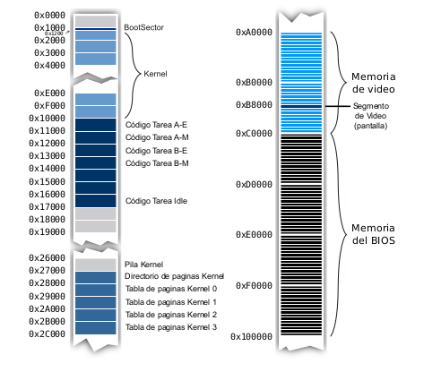
\includegraphics[width=90mm]{ej_3/img_ej_3.png}
\end{figure}

Para esto, en la función \texttt{mmu\_inicializar\_dir\_kernel}. Seteamos la direccion de la page directory en 0x27000 y de la page table 0 en 0x28000 como indica la figura.\\

Luego llamamos a \texttt{mmu\_empty\_mapping} que se encarga de inicializar las entradas 1 a 1024 de la page directory con base 0x00000 y atributos 0x00.\\
y a la función \texttt{mmu\_identity\_mapping} que se mapea con identity mapping las entradas 0 a 1024 de la page table, con atributos p=1 y r/w=1.\\
La entrada 0 de la page directory tiene como base la dirección de la page table 0 (0x28000) y atributos p=1 y r/w=1.\\

Una vez creadas estas estructuras, habilitamos la paginación cargando en cr3 la dirección del page directory (0x27000) y seteando en 1 el bit más significativo de cr0.\\


% Fin Ejercicio 3

\newpage	
% Comienzo Ejercicio 4
\section{Ejericio 4}

\subsection{Manejo de memoria para las tareas}

En este ejercicio, con el fin de poder manejar la memoria utilizada por las distintas tareas, creamos tomando como base las sugerencias dadas en el enunciado, las siguientes funciones que permiten inicializar un directorio de páginas para una tarea, así como mapear y desmapear páginas.

Rutina \texttt{inicializar\_mmu} para administrar la memoria en el área libre. Esta función setea la variable global next\_page en la primer página no usada (\texttt{AREA\_LIBRE} = 0x100000). 

\texttt{mmu\_inicializar\_dir\_pirata}  donde pedimos una nueva pagina para el directorio de páginas y seteamos en su primer entrada la tabla del kernel con p=1 y r/w=1. Luego mapeamos la pagina de codigo (0x400000) con la posicion fisica del pirata en el mapa y copiamos el codigo pertinente del pirata que corresponde. Además se mapean todas las posiciones ya exploradas por el jugador.

Para esto inicializamos una page directory nueva, ya que cada tarea dispondrá de la suya propia. Con este fin, en primer lugar pedimos una página libre con \texttt{mmu\_new\_page} que da la dirección a la próxima página a mapear libre. Luego hacemos empty mapping sobre sus entradas.
La primer entrada será usada para mapear el kernel, por lo tanto pone el código como su base, la setea en presente y con permisos de supervisor.
A continuación mapeamos la página del código. Para esto vamos a cambiar el cr3 (previamente lo guardamos para no perderlo haciendo uint cr3 = rcr3) y hacemos \texttt{mmu\_mapear\_pagina} pasando como parámetros la dirección en la que va a estar el código del pirata (0x400000) y el área del mapa en la cuál está la tarea. Es decir, mapea el área del mapa en donde está la tarea a 0x400000. 
De esta forma, $game_xy2lineal(p->coord.x, p->coord.y) * PAGE_SIZE + MAPA_BASE_FISICA$ es nada más una traducción a la dirección física del mapa correspondiente a la posición (x, y) del pirata.

\texttt{mmu\_copiar}recibe una dirección fuente y una destino (como punteros a unsigned int) y copia el contenido de una en la otra.
Esto se concreta a través de un simple "for" que itera por ambas páginas, asignando fuente[i] a destino[i]. Como el tamaño de una página es 4096 y se va copiando de a 4 bytes, el número de iteraciones es 1024. Con esta función que recibe como dirección fuente el código específico de la tarea y como dirección destino la 0x400000 copiamos el código a la dirección mapeada previamente.


Por ultimo se mapean todas las pocisiones del mapa que fueron exploradas por el jugador específico al pirata. 


\texttt{mmu\_mapear\_pagina} permite mapear la página física en la dirección virtual pasada como parámetros, utilizando cr3. Para esto, recibimos el cr3 y a partir de este obtenemos la dirección de la page directory. Del parámetro virtual obtenemos el offset para la entrada en la page directory y de la page table. Si la entrada de page directory no está presente, creamos una nueva página y para esta entrada, hacemos \texttt{empty\_mapping} sobre las 1024 entradas, es decir, las seteamos como no presentes.
Luego, para la entrada correspondiente al offset de page directory, ponemos como base la dirección de la página creada, y atributos 0x03. 
Finalmente, obtenemos la dirección de la tabla creada y para el offset calculado inicialmente, ponemos como base la dirección física, y como atributos permisos de usuario, presente habilitado y lectura/escritura o solo lectura según corresponda.

\texttt{mmu\_unmapear\_pagina} borra el mapeo creado en la dirección virtual utilizando cr3. Par esto, como en \texttt{mmu\_mapear\_pagina}, calculamos el offset de directorio y tabla a partir de la dirección virtual. Luego, si la entrada correspondiente no existe, significa que ya se encontraba desmapeada y no hacemos nada. Caso contrario, limpiamos las entradas de page directory y page table correspondiente, seteando en 0 el bit de presente.
% Fin Ejercicio 4

\newpage	
% Comienzo Ejercicio 5
\section{Ejericio 5}
\subsection{Rutinas de atención de interrupciones}

En este punto, se nos encarga desarrollar las rutinas de atención de interrupciones para las distintas entradas de la IDT, en particular, la del reloj, la del telcado y la 0x46.

Como en este punto se nos pide el desarrollo de algunas funcionalidades que en los puntos posteriores son reemplazadas por otra, desarrollaremos en este punto el resultado final de las distintas rutinas, tal como se ven en el código terminado.

\subsubsection{Rutina de interrupción del reloj}

Cada vez que se llama a la interrupción del reloj ante cada tick, se llama a la función \texttt{sched\_tick}, quien realiza un llamado a game\_tick y además devuelve lo obtenido tras el llamado a \texttt{sched\_proxima\_a\_ejecutar} que es la próxima tarea a ejecutarse.
La función \texttt{game\_tick} llama a \texttt{screen\_actualizar} que pinta en pantalla los puntos de cada jugador, además de mostrar el reloj global del juego rotando, y el reloj particular del pirata actual, rotando debajo de su número indicador correspondiente, como indica la figura. Para los piratas no activos o muertos, se muestra una cruz.


\begin{figure}[ht]
\centering
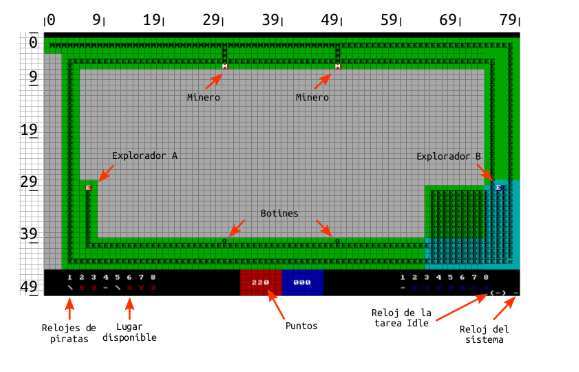
\includegraphics[width=90mm]{ej_5/img_ej_5.png}
\end{figure}


Además, si el jugador tiene mineros disponibles (es decir, tiene mineros para mandar, que se acumularon después de que un explorador descubriese un botín) y la cantidad de piratas vivos del jugador actual es menor a 8, se lanza un pirata minero con la función \texttt{game\_jugador\_lanzar\_pirata}. En esta función se inicializa un pirata a través de \texttt{game\_pirata\_inicializar} que primero busca cuál es el próximo id disponible para el pirata de un jugador, y luego inicializa los campos del struct pirata.
Después se inicializan las entradas de TSS y GDT correspondientes para el pirata a lanzarse con las funciones \texttt{tss\_inicializar\_pirata} y \texttt{gdt\_inicializar\_pirata} descritas en detalle en el punto siguiente y se pinta al pirata en pantalla con la función \texttt{screen\_pintar\_pirata}.
Luego actualizamos las variables del juego, aumentando la cantidad de piratas del jugador, y si el pirata lanzado es un explorador se aumenta la cantidad de exploradores del jugador actual
Si es minero cambiamos el cr3 actual por el cr3 del minero obtenido de su TSS para obtener del stack del minero las direcciones destinadas a botín x e y, y las actualizamos con la posición del botín del jugador.
Finalmente, se restaura el viejo cr3 y decrementa en uno la cantidad de mineros disponibles del jugador, ya que ahora tiene uno menos para mandar.


En la función \texttt{sched\_proxima\_a\_ejecutar} utilizamos la función auxiliar \texttt{sched\_proximo\_pirata}, que recibe un id de jugador y id de pirata y se fija para ese jugador, cual es el siguiente al pirata dado que está vivo y lo devuelve. En caso de que no haya ninguno, se devuelve -1.

Luego, se chequea, en primer caso, si no hay ninguna tarea activa para ningún jugador (es decir, el llamado para \texttt{game\_proximo\_pirata} para ambos jugadores con el pirata actual dio -1), devuelve el índice en GDT de la tarea Idle.

Sino, se llama a \texttt{game\_proximo\_pirata} con ambos jugadores y el pirata actual y se determina para cada jugador, cual es el próximo pirata a ejecutarse, en caso de que tenga uno, y se setea la proxima tarea a ejecutarse según cual sea el jugador actual (en este caso, la siguiente del otro jugador) o según el otro jugador no tenga tareas para ejecutar (en este caso, la siguiente del jugador con tareas). 

Finalmente, con lo devuelto por \texttt{sched\_tick} (el indice en GDT de la próxima tarea a ejecutarse) seteamos el valor del selector en [sched\_tarea\_selector] y realizamos un jmp far a [sched\_tarea\_offset] definidos previamente como sched\_tarea\_offset: dd 0x00 sched\_tarea\_selector: dw 0x00 en la sección de datos, completando el task switch.

\subsubsection{Rutina de atención del teclado}

Para la atención del teclado, en la rutina leemos la tecla que fue presionada y con esta llamamos a \texttt{game\_atender\_teclado}, que en caso de recibir la tecla Shift Left o Shit Right lanza al pirata correspondiente. Además, en caso de que sea la tecla Y, setea el modo debug según corresponda.

\subsubsection{Rutina de atención de las syscalls (\_isr70)}

En la rutina \texttt{\_isr70} llamamos a la función \texttt{game\_syscall\_manejar} con el número de syscall recibida, para luego realizar las distintas rutinas según sea necesario. Las distintas rutinas son:

\begin{enumerate}

	\item \texttt{game\_syscall\_pirata\_mover} que recibe como parámetros un id de pirata y una dirección a la cual debe moverse, que se basa en un enum que tiene los valores ABA, ARR, IZQ, DER.
	Para poder manejar la dirección pasada como parámetros de la misma forma en la que tratamos a las coordenadas de los piratas, convertimos la dirección a un struct coord con la función \texttt{game\_dir2coord}. Una vez realizada la conversión, con la función \texttt{game\_posicion\_valida}, comprobamos que la posición a la que queremos movernos esté dentro de los límites del mapa. Si no lo está, retornamos sin realizar ningún movimiento. Caso contrario, actualizamos la posición del pirata. Si el pirata es explorador, y la posición no había sido previamente explorada por éste, llamamos a \texttt{game\_habilitar\_posicion} que es una función que para cada posición alrededor del explorador, incluyendo a la actual, si ésta no fue explorada la marca como explorada y la mapea. Además, chequea si hay tesoro en esa posición, y de ser así, incrementa en uno la cantidad de mineros del jugador ya que en el próximo \texttt{game\_tick} deberá lanzarse un minero. Además se guarda en el botín del jugador la coordenada recién habilitada.


	\item \texttt{game\_syscall\_cavar} recibe un id de pirata. Si este no corresponde a un minero, retornamos sin realizar ninguna acción.
	Si es minero, llamamos a \texttt{game\_buscar\_botin} con el pirata para ver si en la posición dada hay un botin. Si lo hay pero el valor del tesoro, calculado con \texttt{game\_valor\_tesoro} es 0, se libera al minero, mientras que si el valor es mayor a 0, se suma uno a la cantidad de monedas del jugador que mando la syscall y se resta uno al botín de la posición.

	\item \texttt{game\_syscall\_pirata\_posicion} recibe como parámetro el id del pirata que llama a la syscall y el id del pirata del cuál se quiere conocer la posición. Si el id del pirata del cual se quiere conocer la posición es -1, se devuelve la posición del jugador que llama a la syscall, caso contrario, se devuelve la posición del pirata cuyo id fue pasado por parámetro.

\end{enumerate}

% Fin Ejercicio 5

\newpage	
% Comienzo Ejercicio 6
\section{Ejericio 6}
\subsection{Inicialización de descriptores de TSS en GDT}

En este punto, se nos pide definir las entradas en la GDT para ser usadas como descriptores de TSS a ser utilizadas para las tareas.\\

En la entrada 14 tenemos el descriptor de TSS de la tarea inicial. Para este, seteamos como límite 0x67 y como base, la dirección \texttt{\&tss\_inicial}, con tipo 0x09 (Execute only accessed), el bit de presente habilitado, dpl 0 y granularidad 0.\\

En la entrada 15, el descriptor de la TSS de la tarea idle, tiene los mismos atributos, excepto que la base es \texttt{\&tss\_idle}.\\

Para la inicialización de las entradas de la GDT correspondientes a las tareas piratas, creamos una función gdt\_inicializar\_pirata que dado un un indice y una dirección de TSS, crea una entrada de gdt en la posición gdt[índice] que tiene como base la dirección de TSS, dpl 3, tipo 0x09 (Execute only accessed), límite 0x67, bit de presente en 1 y granularidad 0. Esta función será llamada al momento de lanzar un pirata con el offset correspondiente al jugador y número de tarea a lanzar, y la dirección de la tss inicializada previamente en la función \texttt{tss\_inicializar\_pirata} que será descrita a continuación.


\subsection{Inicialización de TSS}

A continuación, se nos pidió completar la entrada de TSS correspondiente a la tarea Idle.\\

Para esto implementamos la función \texttt{tss\_inicializar} que completa los distintos campos, entre ellos el cr3, cargando el cr3 actual, los flags activados, el eip con la dirección 0x16000, que es donde según el enunciado se encuentra la tarea idle. El esp y ebp en 0x27000, dirección donde se encuentra el directorio de páginas de kernel, y donde cs es el segmento de código de nivel de supervisor, es, dd, ds, gs el segmento de datos de nivel supervisor y fs es el segmento de video.\\

Luego, para completar una TSS libre con los datos de una tarea utilizamos la función \texttt{tss\_inicializar\_pirata} mencionada anteriormente, en la quedado un id de jugador y un id de pirata, obtenemos un puntero a la tss correspondiente a dicha tarea y completamos sus campos. Los flags activados, como eip la dirección 0x400000 (CODIGO\_BASE), que es donde se encuentra el código respectivo de la tarea, esp es \texttt{CODIGO\_BASE+PAGE\_SIZE-12} y ebp \texttt{CODIGO\_BASE+PAGE\_SIZE-12}. El campo cs corresponde al selector de segmento de código de nivel de usuario, mientras que es, ss, ds y fs al de datos de nivel de usuario. Todos los registros son inicializados en 0.\\

Para el cr3 se llama a \texttt{mmu\_inicializar\_dir\_pirata}, que fue detallada anteriormente y para  esp0 a  se pide una página para la pila de nivel 0 con \texttt{mmu\_new\_page} . Ss0 corresponde también al segmento de datos a nivel supervisor. Como anticipamos, esta función es llamada desde \texttt{game\_jugador\_lanzar\_pirata} antes de inicializar el descriptor de GDT de dicha tarea.\\

\subsection{Task switch entre tarea inicial e Idle}

Para saltar intercambiando tareas entre la inicial y la idle, en kernel.asm primero definimos en la sección de datos a selector y offset como un word y double word respectivamente.\\

Antes de pasar a la tarea idle, es necesario cargar la tarea inicial, haciendo uso de la instrucción \texttt{ltr} que la carga en el task register.\\

Luego para hacer el intercambio de tareas entre la inicial y la idle, escribimos un código que mueve el selector de segmento correspondiente a la entrada de la gdt de la tarea idle a [selector] (índice 14) y luego hacemos un jmp far a [offset]. El jump far produce el task switch que permite realizar el intercambio de tareas.


% Fin Ejercicio 6

\newpage	
% Comienzo Ejercicio 7
\section{Ejericio 7}

\subsection{Scheduler, debugger y etcs}

En este punto, se nos pide inicializar las estructuras necesarias para el scheduler. Para esto, tenemos la función \texttt{sched\_inicializar} que setea como jugador actual al jugador A, y como pirata actual de ambos jugadores al 0.\\

Las funciones \texttt{sched\_tick}, \texttt{game\_proximo\_pirata} y \texttt{sched\_proxima\_a\_ejecutar}, también implementadas en este punto, fueron detalladas anteriormente, así como también el desarrollo de la rutina de la interrupción 0x46 para que atienda los servicios de mover, cavar y dar la posición de un pirata.\\

Por último, implementamos el mecanismo de debugging pedido en el enunciado, en el que al presionar la tecla Y se accede al modo debug, y en cuanto se produzca una excepción se mostrará en pantalla el estado del procesador tal como se muestra en la figura.\\

\begin{figure}[ht]
\centering
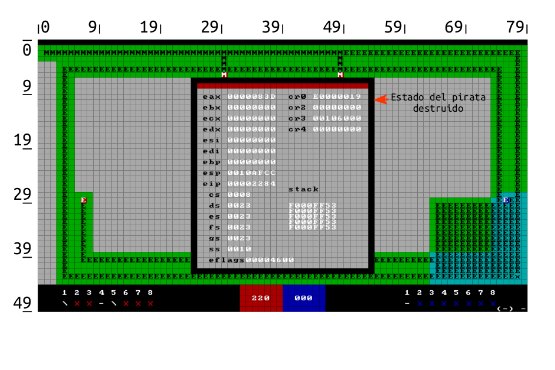
\includegraphics[width=90mm]{ej_7/img_ej_7.png}
\end{figure}

Al presionar nuevamente la tecla Y, se borra la información presentada en pantalla y se desaloja la tarea que produjo la excepción y se salta a la tarea Idle hasta que se decida en el próximo ciclo de reloj cual es la próxima tarea a ser ejecutada.\\

Para realizar esto, en la macro realizada para las excepciones de la 1 a la 19, se chequea si nos encontramos en el modo debug. De no ser así, desalojamos a la tarea que causo la excepcion silenciosamente. Si estábamos en modo debug, se salva el estado actual de la pantalla con \texttt{screen\_pantalla\_debug} y se queda ciclando hasta que se detecte que se presionó nuevamente la tecla Y.\\

Cuando esto suceda, se llama a \texttt{load\_screen} que restablece la pantalla previa y a continuación se llama a \texttt{game\_pirata\_exploto}, que setea al pirata actual como muerto, y resta uno a la cantidad de piratas del jugador correspondiente. A su vez, setea el bit de presente del descriptor en GDT del pirata muerto como 0 y actualiza el reloj del pirata en la pantalla con \texttt{screen\_actualizar\_reloj\_pirata}.\\ 

Finalmente se setea como próximo selector al de la tarea Idle y se realiza un jmp far a esta.\\

El flag de modo debug se setea en 0 o 1 (de acuerdo al valor previo del flag) en \texttt{game\_atender\_teclado} cuando se detecta que la tecla presionada fue Y.\\

La función \texttt{screen\_pantalla\_debug} salva el estado inicial de la pantalla con \texttt{save\_screen} y printea en pantalla la pantalla de debug según se muestra en la ilustración, con los datos correspondientes para la tarea que lanzó la excepción.\\

Como cuando se lanza una excepción de una tarea nivel que está corriendo en nivel 3 se cambia el nivel de privilegio y este pasa a ser 0, se guardan en el stack varios parámetros que usaremos para mostrar en pantalla de debug, ya que estos argumentos obtenidos de la pila son usados como sus parámetros. Además, como utilizamos la instrucción pushad antes de llamar a la función, guardamos en la pila todos los registros de propósito general. 



% Fin Ejercicio 7

\end{document}